\documentclass[11pt,a4paper]{article}

\usepackage[margin=2.3cm]{geometry}
\usepackage{amsmath,amssymb}
\usepackage{graphicx}
\usepackage{booktabs}
\usepackage{xcolor}
\usepackage{enumitem}
\usepackage[hidelinks]{hyperref}
\usepackage{caption}

\emergencystretch=1.5em
\captionsetup{font=small,labelfont=bf,width=.92\textwidth}
\setlength{\parskip}{4pt plus 1pt}
\setlength{\parindent}{0pt}

\newcommand{\code}[1]{\texttt{#1}}
\newcommand{\bst}[1]{\textbf{#1}}

\title{Permuting the surrogate signal\\[2pt]
\large Research note: is $dL/dp_i$ better than its own random permutation?}
\author{}
\date{2026-09-27.}

\begin{document}
\maketitle
\vspace{-2em}

% ============================================================
\section{Purpose and summary of conclusions}
% ============================================================

The RBLapSum backward is not the derivative of its hard forward, which admits
the suspicion that the surrogate gradients it produces are ``wrong'' -- that
the score path works through its scale and structure rather than through the
task signal it routes. This note tests that suspicion with a matched-marginals
control. A fraction $\rho$ of each token's Top-$(K{+}J)$ pool is sampled every
training backward, and the $dL/dp_i = u_i z_i$ values at those positions are
shuffled by a uniform random permutation of the subset -- \emph{before} the
kernel weighting, so every position keeps its own $\kappa_i$, the
$\kappa$-weighted zero-sum correction applies to the permuted signal, and the
hard task path is untouched. The construction preserves the surrogate's scale
profile, kernel locality, zero-sum structure and the per-token multiset of
signal values; it destroys only the \emph{assignment} of signal to neuron.
$\rho = 0$ is bit-for-bit the unmodified backward
(\code{rblapsum\_rho\_random\_perm\_prob\_grad}, training only).

Conclusions:

\begin{itemize}[leftmargin=1.4em]
\item \textbf{The assignment is the signal.} Final CE degrades monotonically
in $\rho$ at both completed windows: $+0.038/+0.076/+0.292$ nats at
$(K,J)=(32,224)$ and $+0.012/+0.066/+0.236$ at $(32,480)$ for
$\rho = 0.25/0.5/1$. Even a quarter of the pool permuted costs a measurable
amount from the first thousand steps, and the gap never closes.

\item \textbf{Fully permuted signal is worse than no surrogate at all.} At
$\rho = 1$ the runs end at $1.7925$ and $1.7269$, clearly above the plain
hard Top-32 baseline ($1.6162$, no surrogate, no output norm). Correctly
scaled, correctly localized, zero-sum noise delivered through the full
surrogate machinery actively damages training; it does not merely waste the
term.

\item \textbf{Narrow windows destabilize under full permutation.} The
$\rho = 1$ cells at $J = 32$ and $J = 96$ were at CE $7.7$ (step 1500) and
$6.0$ (step 2500) and climbing when the campaign was stopped, while the same
$\rho$ survives 20k steps at $J = 224$ and $480$. A wider pool spreads the
same misassigned budget over more candidates, which is consistent with the
boundary-concentration mechanism of the earlier stability work.

\item \textbf{The $\rho = 0$ controls reproduce their ancestors.} $1.4910$
against $1.4943$ at $(32,480)$ and $1.5006$ against $1.4842$ at $(32,224)$ --
$-0.003$ and $+0.016$ nats on different hardware and a newer torch stack,
within this project's single-seed spread. Together with the bitwise unit
test of the $\rho = 0$ code path, the recent codebase changes leave the
baseline intact.
\end{itemize}

The answer to the motivating question is therefore no: the surrogate's
per-neuron credit assignment is its active ingredient. What survives
permutation -- the budget, the kernel geometry, the zero-sum structure -- is
worth less than nothing on its own.

% ============================================================
\section{Setup}
% ============================================================

Sixteen runs on a fresh 8-GPU machine: $K = 32$,
$J \in \{32, 96, 224, 480\}$, $\rho \in \{0, 0.25, 0.5, 1.0\}$, all
\code{through\_rank\_kappa} at $T = 2$ with no output norm, $b_0 = 0$, full
magnitude--direction decoupling, 20k steps. Every run inherits the dumped
\code{config.json} of its ancestor from the earlier campaigns (the
stabilization campaign's $T=2$ arm at $J = 32$ and $480$, the
Top-$(K{+}J)$ campaign's at $J = 96$ and $224$) with only $\rho$ overridden,
so architecture, data, optimizer, schedules and seed are identical to the
references by construction.

The permutation: per (token, block) row, per backward,
$\mathrm{round}(\rho \cdot (K{+}J))$ positions sampled uniformly without
replacement, values shuffled by a uniform permutation of the subset, fresh
randomness every step; evaluation is never permuted. The four wide-window
cells ($J = 224, 480$) ran to completion; the eight narrow-window cells were
stopped by hand at steps 1500--3500 to free the machine once the wide cells
had settled the ordering -- their curves are reported as observed, and none
had been stopped by the divergence guard at that point.

% ============================================================
\section{Results}
% ============================================================

Final validation CE after 20k steps (completed cells), with the gap to the
unpermuted run of the same cell:

\begin{center}\small
\begin{tabular}{lcccc}
\toprule
$(K,J)$ & $\rho=0$ & $\rho=0.25$ & $\rho=0.5$ & $\rho=1$ \\
\midrule
$(32,224)$ & \bst{1.5006} & 1.5381 ($+0.038$) & 1.5761 ($+0.076$) & 1.7925 ($+0.292$) \\
$(32,480)$ & \bst{1.4910} & 1.5025 ($+0.012$) & 1.5566 ($+0.066$) & 1.7269 ($+0.236$) \\
\midrule
\multicolumn{5}{l}{hard Top-32, no surrogate (reference): 1.6162} \\
\bottomrule
\end{tabular}
\end{center}

The degradation is monotone in $\rho$ at both windows and visibly ordered
from about step 1000 onward. At $\rho = 1$ both cells end $0.11$--$0.18$
nats \emph{above} the no-surrogate baseline. Partial permutation degrades
sublinearly at $J = 480$ ($\rho = 0.25$ costs little) and closer to linearly
at $J = 224$.

The stopped narrow-window cells, last validation before the stop:

\begin{center}\small
\begin{tabular}{lcccc}
\toprule
$(K,J)$ & $\rho=0$ & $\rho=0.25$ & $\rho=0.5$ & $\rho=1$ \\
\midrule
$(32,32)$ & 1.9615 (2500) & 2.0313 (2500) & 2.2246 (2000) & 7.6565 (1500) \\
$(32,96)$ & 1.8389 (3500) & 1.9070 (3500) & 2.0603 (3000) & 5.9900 (2500) \\
\bottomrule
\end{tabular}
\end{center}

The same monotone ordering holds at every observed step, and the $\rho = 1$
cells are not merely behind but diverging -- CE 6--8 and rising -- where the
wide-window $\rho = 1$ cells train stably to the end.

\begin{figure}[htb]\centering
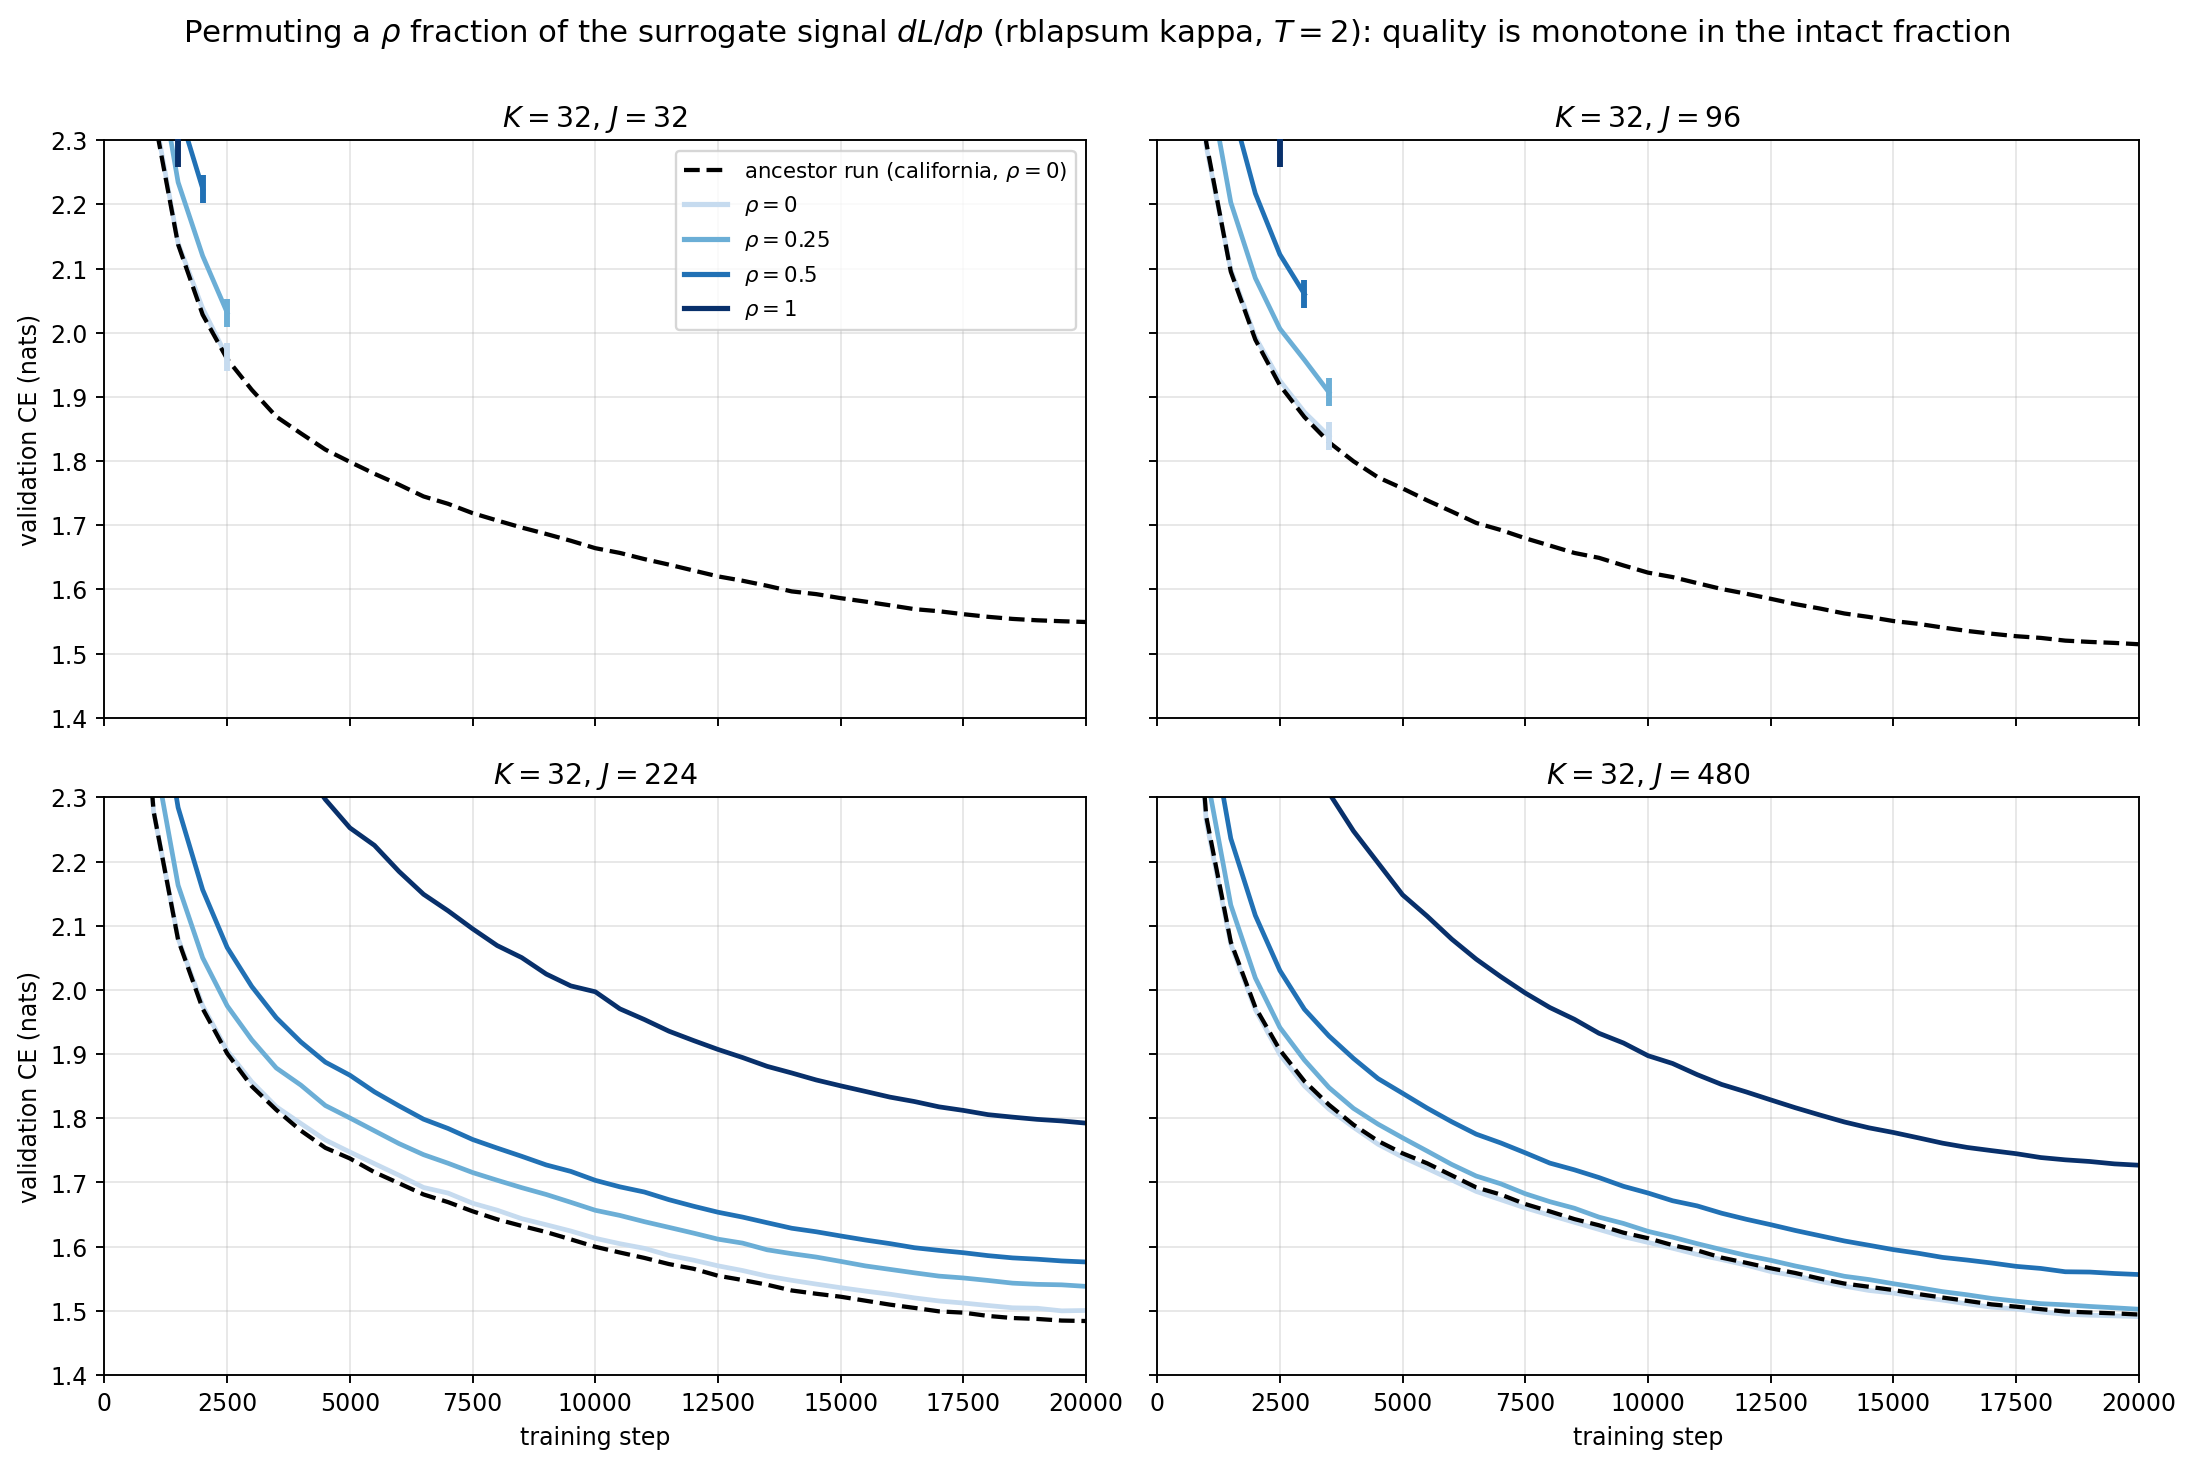
\includegraphics[width=\textwidth]{figures/rho/rho_perm_by_j.png}
\caption{Validation CE by window, $\rho$ light to dark, the california
ancestor of each cell dashed. In the completed panels (bottom) the
$\rho = 0$ curve lies on its ancestor and the ordering in $\rho$ is
monotone throughout; in the stopped panels (top) the tick marks the last
measurement, with $\rho = 1$ already above the axis range and climbing.}
\end{figure}

\paragraph{The control.}
$\rho = 0$ against the ancestor run of the same cell: $1.4910$ vs $1.4943$
at $(32,480)$, $1.5006$ vs $1.4842$ at $(32,224)$. The first agrees to
$0.003$ nats; the second differs by $+0.016$, at the upper end of the
run-to-run variation this project has seen from identical configs across
machines, and the two curves track each other throughout training. Since the
$\rho = 0$ code path is additionally covered by a bitwise identity test, we
read both as agreement: the sf, value-gradient, permutation and
data-parallel changes to the codebase did not move the baseline.

% ============================================================
\section{Interpretation}
% ============================================================

The control was designed so that everything except credit assignment
survives: each permuted position still receives a correctly-scaled,
correctly-localized kick, each token still injects the same multiset of
signal values into the same kernel profile, and the correction still removes
the common mode. If the surrogate worked through its budget or its geometry,
$\rho = 1$ would approximately reproduce it. Instead $\rho = 1$ is worse
than deleting the term entirely, which pins the surrogate's value -- and
more -- on \emph{which neuron gets which signal}.

That full permutation is worse than nothing admits a mechanical reading
consistent with the earlier scale-dynamics measurements, though we mark it
as interpretation. The misassigned kicks are refreshed every step, so their
first-order effect averages toward zero; what does not average out is
second-order: every step executes full-magnitude updates on wrongly-chosen
rows (Adam normalizes per parameter, so a persistent stream of large
misassigned gradients produces full-size steps), which is pure heating of
the score scale plus a per-step scrambling of the ranking the forward
depends on. The narrow-window divergences fit the same picture: at
$J = 32$ the permuted budget lands on 64 candidates instead of 512, the
per-neuron kick is an order of magnitude larger, and the boundary-referenced
geometry that the kappa-ablation note showed to be the fragile quantity is
kicked correspondingly harder.

For the programme, the positive statement is the useful one: the RBLapSum
backward, non-derivative as it is, carries real per-neuron task information
-- the ``wrong gradients'' hypothesis is rejected in its strong form. The
cheap follow-up, not run, is the same sweep on the boundary term alone
(permuting only the $-q\,\Sigma a$ routing while leaving the direct term
intact), which would split the credit between the two components of the
score path.

% ============================================================
\section{Scope}
% ============================================================

Single runs at one seed, one active count ($K = 32$), one variant ($T = 2$,
no output norm), and a coarse $\rho$ grid. The narrow-window cells are
truncated at steps 1500--3500 by an operational decision, not by the guard:
their divergence-in-progress at $\rho = 1$ is an observation about
trajectories, not recorded final outcomes, and earlier work found
marginal-cell divergence stochastic. The ancestors were trained on a
different machine and torch version, so the control comparison inherits
cross-machine variation ($\pm 0.01$--$0.02$ nats). The permutation acts
before the kernel weighting by design; the harsher post-$\kappa$ variant
(scrambling the scale profile along with the signal) was specified but not
run, and the permutation of the boundary routing alone was not attempted.

\end{document}
